\documentclass[9pt,a4paper]{article}
\usepackage[margin=1.8cm,top=2.0cm,bottom=2.0cm]{geometry}
\usepackage{booktabs,colortbl,xcolor,array,makecell,hhline}
\usepackage{amsmath,amssymb}
\usepackage{helvet}\renewcommand{\familydefault}{\sfdefault}
\usepackage{fancyhdr,graphicx}
\usepackage[colorlinks=true,linkcolor=primary,urlcolor=primary,
            bookmarks=true,pdfborder={0 0 0}]{hyperref}
\usepackage{parskip,enumitem,titlesec,needspace}
\setlength{\parskip}{2pt}
\definecolor{passgreen}{RGB}{198,239,206}
\definecolor{failred}{RGB}{255,199,206}
\definecolor{warnamber}{RGB}{255,235,156}
\definecolor{r2green}{RGB}{198,239,206}
\definecolor{r2amber}{RGB}{255,235,156}
\definecolor{primary}{RGB}{0,70,127}
\definecolor{sepgray}{RGB}{130,130,130}
\titleformat{\section}{\normalsize\bfseries\color{primary}}{}{0em}{}
            [\vspace{-4pt}\textcolor{primary}{\rule{\linewidth}{0.5pt}}]
\titlespacing{\section}{0pt}{16pt}{6pt}
\newcommand{\exhead}[1]{%
  \medskip\noindent{\small\bfseries\color{primary}#1}%
  \par\vspace{-5pt}\noindent\textcolor{primary}{\rule{\linewidth}{0.4pt}}\vspace{2pt}}
\pagestyle{fancy}\fancyhf{}
\lhead{\small\textcolor{primary}{\textbf{Surrogate Factory}}}
\chead{\small\textcolor{sepgray}{CONFIDENTIAL}}
\rhead{\small\textcolor{primary}{UCHARDLANDING\_1}}
\lfoot{\small\textcolor{sepgray}{Surrogate Factory v2.2 --- Automated Validation Report}}
\rfoot{\small\thepage}
\renewcommand{\headrulewidth}{0.4pt}\renewcommand{\footrulewidth}{0.4pt}
\begin{document}
% ==== EXECUTIVE SUMMARY ====
\thispagestyle{fancy}

\begin{center}
  {\large\bfseries\color{primary} Executive Summary --- Surrogate Model Validation Report}\\[2pt]
  {\small\color{sepgray} Use case: \textbf{UCHARDLANDING\_1} \quad|\quad 09 September 2026 \quad|\quad 2 model(s)}
\end{center}
\vspace{-4pt}\noindent\rule{\linewidth}{1pt}\vspace{3pt}

\begin{center}
\colorbox{passgreen}{\begin{minipage}{0.66\linewidth}
  \vspace{5pt}\centering
  {\normalsize\bfseries ALL REQUIREMENTS MET}\\[4pt]
  {\small\bfseries Recommended model:} {\small GradientBoosting}\\[5pt]
\colorbox{r2green}{\begin{minipage}{0.97\linewidth}\vspace{2pt}\centering {\small\bfseries Avg R\textsuperscript{2}: 0.9836} \enspace---\enspace {\small Excellent}\vspace{2pt}\end{minipage}}\\[2pt]
\colorbox{passgreen}{\begin{minipage}{0.97\linewidth}\vspace{2pt}\centering {\small\bfseries Q90 Accuracy} \enspace---\enspace {\small All outputs pass}\\[1pt]{\footnotesize Pass: O1, O2}\vspace{2pt}\end{minipage}}
  \vspace{5pt}
\end{minipage}}
\end{center}

\section{Project Overview}
\renewcommand{\arraystretch}{1.2}
\begin{tabular}{|l|p{0.60\linewidth}|}
  \hline
  \textbf{Use case}           & UCHARDLANDING\_1 \\ \hline
  \textbf{Inputs}             & I1, I2, I3, I4, I5, I6, I7 \\ \hline
  \textbf{Outputs}            & 2: O1, O2 \\ \hline
  \textbf{Train / Val / Test} & 80\% / 10\% / 10\% \\ \hline
  \textbf{Accuracy target}    & Q90 $<$ 10\% relative error per output \\ \hline
\end{tabular}

\par\begin{minipage}{\linewidth}
\section{Variable Correlation --- Input vs Output}
\begin{center}
\includegraphics[width=0.80\linewidth,height=0.46\textheight,keepaspectratio]{analysis_plots/data_scatter_vars.png}\end{center}
\end{minipage}\par\medskip
\section{Data Statistics}
Per-variable statistics over all data (train + val + test), as \texttt{Train\_set.describe()} reports them in the feature-selection notebook: count, mean, standard deviation, minimum, quartiles and maximum.

\par\begin{minipage}{\linewidth}
\exhead{Inputs}
\begin{center}
\footnotesize
\renewcommand{\arraystretch}{1.15}
\resizebox{\linewidth}{!}{%
\begin{tabular}{|l|r|r|r|r|r|r|r|r|}
\hline
\textbf{} & \textbf{count} & \textbf{mean} & \textbf{std} & \textbf{min} & \textbf{P25} & \textbf{P50} & \textbf{P75} & \textbf{max} \\ \hline
\textbf{I1} & 89,357 & 0.5276 & 0.2292 & 0.1646 & 0.3292 & 0.4938 & 0.679 & 1 \\ \hline
\textbf{I2} & 89,357 & 0.3137 & 0.2394 & 0 & 0.0909 & 0.2727 & 0.4545 & 0.9636 \\ \hline
\textbf{I3} & 89,357 & 0.4757 & 0.2439 & 0.1538 & 0.2308 & 0.3846 & 0.6923 & 0.9231 \\ \hline
\textbf{I4} & 89,357 & 0.4694 & 0.2875 & 0.1333 & 0.1333 & 0.3333 & 0.5333 & 0.93 \\ \hline
\textbf{I5} & 89,357 & -0.000187 & 0.5404 & -0.6667 & -0.6667 & 0 & 0.6667 & 0.6667 \\ \hline
\textbf{I6} & 89,357 & 0.2577 & 0.4374 & 0 & 0 & 0 & 1 & 1 \\ \hline
\textbf{I7} & 89,357 & 0.3477 & 0.1585 & 0.0042 & 0.2366 & 0.3448 & 0.4558 & 0.8502 \\ \hline
\end{tabular}
}
\par\vspace{2pt}
{\scriptsize Input variables — Train\_set.describe()}
\end{center}
\end{minipage}\par\medskip
\par\begin{minipage}{\linewidth}
\exhead{Outputs}
\begin{center}
\footnotesize
\renewcommand{\arraystretch}{1.15}
\resizebox{\linewidth}{!}{%
\begin{tabular}{|l|r|r|r|r|r|r|r|r|}
\hline
\textbf{} & \textbf{count} & \textbf{mean} & \textbf{std} & \textbf{min} & \textbf{P25} & \textbf{P50} & \textbf{P75} & \textbf{max} \\ \hline
\textbf{O1} & 89,357 & 0.4207 & 0.154 & 0.0511 & 0.3061 & 0.4217 & 0.5289 & 0.9489 \\ \hline
\textbf{O2} & 89,357 & 0.3301 & 0.1204 & 0.0833 & 0.2367 & 0.326 & 0.411 & 0.9167 \\ \hline
\end{tabular}
}
\par\vspace{2pt}
{\scriptsize Output variables — Train\_set.describe()}
\end{center}
\end{minipage}\par\medskip
\section{Model Selection}
\begin{minipage}{\linewidth}
\renewcommand{\arraystretch}{1.2}
\begin{tabular}{|l|r|r|r|}
  \hline
  \textbf{Model} & \textbf{Avg R\textsuperscript{2}} & \textbf{Q90 pass (2)} & \textbf{KS pass (2)} \\ \hline
  {\bfseries GradientBoosting\ $\star$} & {\bfseries 0.9836} & {\bfseries 2/2} & {\bfseries 2/2} \\ \hline
  { MLP} & { 0.9828} & { 2/2} & { 2/2} \\ \hline
\end{tabular}
\par\vspace{4pt}
{\footnotesize $\star$ Recommended model.\enspace Q90 target: $<10\%$.\enspace KS: $p\geq 0.05$ = no overfitting.}
\end{minipage}

\section{Accuracy Assessment (Q90 \& R\textsuperscript{2})}
\begin{minipage}{\linewidth}
\renewcommand{\arraystretch}{1.2}
\begin{tabular}{l|rrr|rrr|}
  \hline
  \textbf{Output} & \multicolumn{3}{c|}{\textbf{GradientBoosting}\ $\star$} & \multicolumn{3}{c|}{\textbf{MLP}} \\ \hline
  & R\textsuperscript{2} & Q90 & Gap & R\textsuperscript{2} & Q90 & Gap \\ \hline
  O1 & \cellcolor{r2green}0.9960 & \cellcolor{passgreen}0.0407 & \cellcolor{passgreen}-0.0593 & \cellcolor{r2green}0.9952 & \cellcolor{passgreen}0.0443 & \cellcolor{passgreen}-0.0557 \\ \hline
  O2 & \cellcolor{r2green}0.9712 & \cellcolor{passgreen}0.0870 & \cellcolor{passgreen}-0.0130 & \cellcolor{r2green}0.9705 & \cellcolor{passgreen}0.0851 & \cellcolor{passgreen}-0.0149 \\ \hline
\end{tabular}
\par\vspace{4pt}
{\footnotesize \colorbox{r2green}{\ } R\textsuperscript{2}$\!\geq\!0.95$\enspace \colorbox{r2amber}{\ } R\textsuperscript{2}$\!\in[0.80,0.95)$\enspace \colorbox{failred}{\ } R\textsuperscript{2}$\!<\!0.80$ or Q90 fail\enspace \colorbox{passgreen}{\ } pass\enspace Gap$=$Q90$-$target ($<\!0\Rightarrow$ margin)}
\end{minipage}

\par\begin{minipage}{\linewidth}
\section{Training History}
\begin{center}
\includegraphics[width=0.70\linewidth,height=0.28\textheight,keepaspectratio]{../training_curve.png}\end{center}
{\footnotesize Training and validation loss per iteration, log scale. The validation curve is measured, not approximated: per epoch on the early-stopping split for the MLP, per stage on the validation split for gradient boosting (whose training curve is its per-stage deviance). Models saved before this was recorded fall back to the $(1-R^2)\cdot\mathrm{Var}(y)/2$ approximation.}\end{minipage}\par\medskip

\par\begin{minipage}{\linewidth}
\section{Predicted vs True --- GradientBoosting}
\begin{center}
\includegraphics[width=\linewidth,height=0.80\textheight,keepaspectratio]{analysis_plots/winner_pred_true.png}\end{center}
\end{minipage}\par\medskip


\section{Data Split Quality}
\begin{minipage}{\linewidth}
\renewcommand{\arraystretch}{1.2}
\begin{tabular}{|l|r|c|}
  \hline\textbf{Metric} & \textbf{Value} & \textbf{Pass} \\ \hline
  Residual voxel proportion ($\leq\!0.05$) & 0.000 & \cellcolor{passgreen}$\checkmark$ \\ \hline
  Valid test proportion & 0.968 & \\ \hline
  p-hacking test proportion ($\leq\!0.05$ warn) & 0.009 & \cellcolor{passgreen}$\checkmark$ \\ \hline
  Isolated test proportion ($\leq\!0.05$ warn) & 0.024 & \cellcolor{passgreen}$\checkmark$ \\ \hline
  Chi\textsuperscript{2} p-value ($\geq\!0.05$) & \textemdash & \textemdash \\ \hline
\end{tabular}
\end{minipage}
\textcolor{passgreen!60!black}{\textbf{No p-hacking concern:}} only 0.9\% of test points lie closer to a training point than training points are to each other, so the test error is not flattered.

\section{Overfitting Check (KS Test) --- GradientBoosting}
\begin{minipage}{\linewidth}
\renewcommand{\arraystretch}{1.15}
\begin{tabular}{|l|r|}
  \hline\textbf{Output} & \textbf{KS p-value} \\ \hline
  O1 & \cellcolor{passgreen}0.074 \\ \hline
  O2 & \cellcolor{passgreen}0.162 \\ \hline
\end{tabular}
\par\vspace{4pt}
{\footnotesize \colorbox{passgreen}{\ } $p\geq 0.05$ --- no overfitting\enspace \colorbox{failred}{\ } $p<0.05$ --- overfitting detected}
\end{minipage}
\clearpage
\thispagestyle{empty}
\vspace*{\fill}
\begin{center}
  \textcolor{sepgray}{\rule{0.40\linewidth}{1pt}}\\[20pt]
  {\Huge\bfseries\color{primary} Deep Analysis}\\[10pt]
  {\large\color{sepgray} UCHARDLANDING\_1}\\[6pt]
  {\normalsize\color{sepgray} Winner Model --- Full Validation}\\[20pt]
  \textcolor{sepgray}{\rule{0.40\linewidth}{1pt}}
\end{center}
\vspace*{\fill}
\clearpage
% ==== PART 3 - DEEP ANALYSIS ====
\label{sec:deepanalysis}
\begin{center}
  {\normalsize\bfseries\color{primary} Deep Analysis --- GradientBoosting}\\[2pt]
  {\small\color{sepgray} Mirrors \texttt{validation\_template.ipynb} --- all computations from validation CSVs}
\end{center}
\vspace{4pt}
\begin{itemize}[leftmargin=2em,itemsep=1pt,topsep=2pt]
  \item \hyperref[sec:d1]{3.1 Data Overview}
  \item \hyperref[sec:d2]{3.2 Train-Test Split Analysis}
  \item \hyperref[sec:d3]{3.3 Error Quantification --- P(E)}
  \item \hyperref[sec:d4]{3.4 P(E|X) --- Error Conditional on Inputs}
  \item \hyperref[sec:d5]{3.5 P(E|Y) --- Error Conditional on Outputs}
  \item \hyperref[sec:d6]{3.6 Uncertainty Analysis}
\end{itemize}

\clearpage
\section{Data Overview}
\label{sec:d1}

Statistical summary of inputs and outputs over all data (train + val + test), as reported by \texttt{describe()} in the feature-selection notebook: count, mean, standard deviation, minimum, quartiles and maximum per variable. All figures in this part are drawn by \texttt{validationlib}, matching the extended validation notebook.

\exhead{Input Statistics}
\begin{center}
\footnotesize
\renewcommand{\arraystretch}{1.15}
\resizebox{\linewidth}{!}{%
\begin{tabular}{|l|r|r|r|r|r|r|r|r|}
\hline
\textbf{} & \textbf{count} & \textbf{mean} & \textbf{std} & \textbf{min} & \textbf{P25} & \textbf{P50} & \textbf{P75} & \textbf{max} \\ \hline
\textbf{I1} & 89,357 & 0.5276 & 0.2292 & 0.1646 & 0.3292 & 0.4938 & 0.679 & 1 \\ \hline
\textbf{I2} & 89,357 & 0.3137 & 0.2394 & 0 & 0.0909 & 0.2727 & 0.4545 & 0.9636 \\ \hline
\textbf{I3} & 89,357 & 0.4757 & 0.2439 & 0.1538 & 0.2308 & 0.3846 & 0.6923 & 0.9231 \\ \hline
\textbf{I4} & 89,357 & 0.4694 & 0.2875 & 0.1333 & 0.1333 & 0.3333 & 0.5333 & 0.93 \\ \hline
\textbf{I5} & 89,357 & -0.000187 & 0.5404 & -0.6667 & -0.6667 & 0 & 0.6667 & 0.6667 \\ \hline
\textbf{I6} & 89,357 & 0.2577 & 0.4374 & 0 & 0 & 0 & 1 & 1 \\ \hline
\textbf{I7} & 89,357 & 0.3477 & 0.1585 & 0.0042 & 0.2366 & 0.3448 & 0.4558 & 0.8502 \\ \hline
\end{tabular}
}
\par\vspace{2pt}
{\scriptsize Input variables — Train\_set.describe()}
\end{center}
\par\begin{minipage}{\linewidth}
\exhead{Input Histograms}
\begin{center}
\includegraphics[width=1.0\linewidth,height=0.80\textheight,keepaspectratio]{analysis_plots/data_input_hist.png}\end{center}
\end{minipage}\par\medskip
\par\begin{minipage}{\linewidth}
\exhead{Input Cumulative Distributions}
\begin{center}
\includegraphics[width=1.0\linewidth,height=0.80\textheight,keepaspectratio]{analysis_plots/data_input_cdf.png}\end{center}
\end{minipage}\par\medskip
\exhead{Output Statistics}
\begin{center}
\footnotesize
\renewcommand{\arraystretch}{1.15}
\resizebox{\linewidth}{!}{%
\begin{tabular}{|l|r|r|r|r|r|r|r|r|}
\hline
\textbf{} & \textbf{count} & \textbf{mean} & \textbf{std} & \textbf{min} & \textbf{P25} & \textbf{P50} & \textbf{P75} & \textbf{max} \\ \hline
\textbf{O1} & 89,357 & 0.4207 & 0.154 & 0.0511 & 0.3061 & 0.4217 & 0.5289 & 0.9489 \\ \hline
\textbf{O2} & 89,357 & 0.3301 & 0.1204 & 0.0833 & 0.2367 & 0.326 & 0.411 & 0.9167 \\ \hline
\end{tabular}
}
\par\vspace{2pt}
{\scriptsize Output variables — Train\_set.describe()}
\end{center}
\par\begin{minipage}{\linewidth}
\exhead{Output Histograms}
\begin{center}
\includegraphics[width=1.0\linewidth,height=0.80\textheight,keepaspectratio]{analysis_plots/data_output_hist.png}\end{center}
\end{minipage}\par\medskip
\par\begin{minipage}{\linewidth}
\exhead{Output Cumulative Distributions}
\begin{center}
\includegraphics[width=1.0\linewidth,height=0.80\textheight,keepaspectratio]{analysis_plots/data_output_cdf.png}\end{center}
\end{minipage}\par\medskip
\clearpage
\section{Train-Test Split Analysis}
\label{sec:d2}

A well-designed split produces training and test distributions that are similar but not identical. The Kolmogorov-Smirnov (KS) test and the Anderson-Darling (AD) test are used to assess distributional similarity. $H_0$: both sets come from the same distribution. $p<0.05$ rejects $H_0$ (undesirable if too low; undesirable if the split was done by stratification and $p$ is too high).

\par\begin{minipage}{\linewidth}
\exhead{Output Distributions: Train vs Test}
\begin{center}
\includegraphics[width=1.0\linewidth,height=0.80\textheight,keepaspectratio]{analysis_plots/split_output_dists.png}\end{center}
\end{minipage}\par\medskip
\par\begin{minipage}{\linewidth}
\exhead{Input Distributions: Train vs Test}
\begin{center}
\includegraphics[width=1.0\linewidth,height=0.80\textheight,keepaspectratio]{analysis_plots/split_input_dists.png}\end{center}
\end{minipage}\par\medskip
\exhead{KS and AD Test Results}
\begin{center}
\footnotesize
\renewcommand{\arraystretch}{1.15}
\begin{tabular}{|l|r|r|}
\hline
\textbf{} & \textbf{KS} & \textbf{AD} \\ \hline
\textbf{O1} & \cellcolor{passgreen}0.684 & \cellcolor{passgreen}0.25 \\ \hline
\textbf{O2} & \cellcolor{passgreen}0.6428 & \cellcolor{passgreen}0.25 \\ \hline
\end{tabular}
\par\vspace{2pt}
{\scriptsize Train vs test p-values. Red: $p<0.05$ (distributions differ).}
\end{center}
\exhead{Split Quality --- Voxel Tesselation Proximity (p-hacking check)}
Beyond matching distributions, a split can still flatter the model if test points sit right next to training points (\textbf{p-hacking}) or probe regions the model never saw (\textbf{isolated}, \textbf{residual voxel}). The VTPM method from \texttt{validationlib} (SF\_9 cell 9.0) classifies every test point.

\begin{minipage}{\linewidth}
\renewcommand{\arraystretch}{1.2}
\begin{tabular}{|l|r|c|}
  \hline\textbf{Metric} & \textbf{Value} & \textbf{Pass} \\ \hline
  Residual voxel proportion ($\leq\!0.05$) & 0.000 & \cellcolor{passgreen}$\checkmark$ \\ \hline
  Valid test proportion & 0.968 & \\ \hline
  p-hacking test proportion ($\leq\!0.05$ warn) & 0.009 & \cellcolor{passgreen}$\checkmark$ \\ \hline
  Isolated test proportion ($\leq\!0.05$ warn) & 0.024 & \cellcolor{passgreen}$\checkmark$ \\ \hline
  Chi\textsuperscript{2} p-value ($\geq\!0.05$) & \textemdash & \textemdash \\ \hline
\end{tabular}
\end{minipage}

\textcolor{passgreen!60!black}{\textbf{No p-hacking concern:}} only 0.9\% of test points lie closer to a training point than training points are to each other, so the test error is not flattered.

\par\begin{minipage}{\linewidth}
\exhead{Error Distribution: Valid vs p-hacking Test Points}
Absolute error of the test points flagged as p-hacking against the valid ones, exactly as the extended validation notebook draws it. Matching distributions (high p-values) mean the flagged points do not distort the reported error.
\begin{center}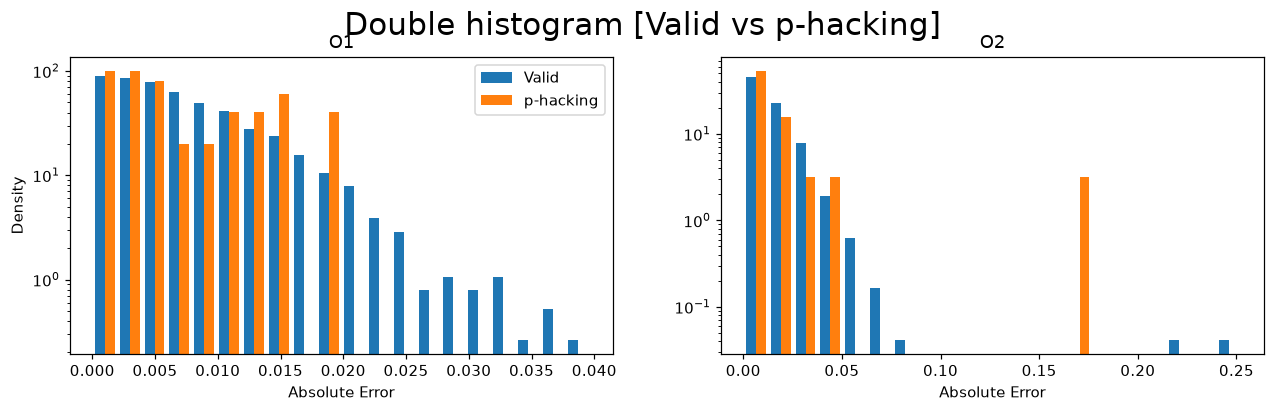
\includegraphics[width=1.0\linewidth,height=0.80\textheight,keepaspectratio]{analysis_plots/phack_hist.png}\end{center}
\begin{center}
\footnotesize
\renewcommand{\arraystretch}{1.15}
\begin{tabular}{|l|r|r|r|}
\hline
\textbf{} & \textbf{AD} & \textbf{KS} & \textbf{KW} \\ \hline
\textbf{O1} & \cellcolor{passgreen}0.25 & \cellcolor{passgreen}0.7073 & \cellcolor{passgreen}0.9937 \\ \hline
\textbf{O2} & \cellcolor{passgreen}0.25 & \cellcolor{passgreen}0.085 & \cellcolor{passgreen}0.2566 \\ \hline
\end{tabular}
\par\vspace{2pt}
{\scriptsize Valid ($n=1922$) vs p-hacking ($n=25$) absolute-error distributions, on a subsample of the test set. Red: $p<0.05$ (the flagged points behave differently).}
\end{center}
\end{minipage}\par\medskip
\par\begin{minipage}{\linewidth}
\exhead{Error Distribution: Valid vs Isolated Test Points}
Same comparison for the test points with no training neighbour.
\begin{center}
\includegraphics[width=1.0\linewidth,height=0.80\textheight,keepaspectratio]{analysis_plots/isolated_hist.png}\end{center}
\begin{center}
\footnotesize
\renewcommand{\arraystretch}{1.15}
\begin{tabular}{|l|r|r|r|}
\hline
\textbf{} & \textbf{AD} & \textbf{KS} & \textbf{KW} \\ \hline
\textbf{O1} & \cellcolor{passgreen}0.2335 & \cellcolor{passgreen}0.143 & \cellcolor{passgreen}0.2572 \\ \hline
\textbf{O2} & \cellcolor{passgreen}0.1288 & \cellcolor{passgreen}0.1172 & \cellcolor{passgreen}0.1187 \\ \hline
\end{tabular}
\par\vspace{2pt}
{\scriptsize Valid ($n=1922$) vs Isolated ($n=53$) absolute-error distributions, on a subsample of the test set. Red: $p<0.05$ (the flagged points behave differently).}
\end{center}
\end{minipage}\par\medskip
\clearpage
\section{Error Quantification --- P(E)}
\label{sec:d3}

Two error metrics are studied:
\begin{itemize}[leftmargin=1.4em,itemsep=1pt,topsep=1pt]
  \item \textbf{Residue:} $e_i = y_i - \hat{y}_i$. A centred ($\mu\approx 0$), symmetric distribution indicates an unbiased model.
  \item \textbf{Absolute Error:} $|e_i|$. Always non-negative; its Q90 must satisfy the accuracy requirement.
\end{itemize}

\exhead{Residue Statistics Table}
Bootstrap confidence bounds shown as superscript (upper) and subscript (lower).
\begin{center}
\footnotesize
\renewcommand{\arraystretch}{1.15}
\resizebox{\linewidth}{!}{%
\begin{tabular}{|l|r|r|r|r|r|r|r|r|r|r|r|r|r|r|r|}
\hline
\textbf{} & \textbf{count} & \textbf{min} & \textbf{max} & \textbf{mean} & \textbf{(BS)mean} & \textbf{median} & \textbf{(BS)median} & \textbf{std} & \textbf{(BS)std} & \textbf{IQR} & \textbf{(BS)IQR} & \textbf{kurtosis} & \textbf{(BS)kurtosis} & \textbf{skewness} & \textbf{(BS)skewness} \\ \hline
\textbf{O1} & 17,872 & -0.0462 & 0.0476 & 4.66e-05 & $^{0.000184}_{\text{-9.85e-05}}$ & 9.86e-05 & $^{0.000231}_{\text{-6.67e-05}}$ & 0.0098 & $^{0.0099}_{0.0096}$ & 0.012 & $^{0.0121}_{0.0117}$ & 0.7 & $^{0.823}_{0.59}$ & -0.0602 & $^{-0.0148}_{-0.118}$ \\ \hline
\textbf{O2} & 17,872 & -0.0848 & 0.449 & 0.000286 & $^{0.000586}_{\text{-3.35e-05}}$ & -0.000407 & $^{-0.000115}_{-0.000645}$ & 0.0205 & $^{0.0215}_{0.0193}$ & 0.0209 & $^{0.0213}_{0.0205}$ & 63.8 & $^{89.1}_{31.2}$ & 4.09 & $^{5.22}_{2.43}$ \\ \hline
\end{tabular}
}
\par\vspace{2pt}
{\scriptsize Residue statistics with bootstrap confidence intervals (superscript/subscript bounds).}
\end{center}
\exhead{Absolute Error Statistics Table}
\begin{center}
\footnotesize
\renewcommand{\arraystretch}{1.15}
\resizebox{\linewidth}{!}{%
\begin{tabular}{|l|r|r|r|r|r|r|r|r|r|r|r|r|r|r|r|}
\hline
\textbf{} & \textbf{count} & \textbf{min} & \textbf{max} & \textbf{mean} & \textbf{(BS)mean} & \textbf{median} & \textbf{(BS)median} & \textbf{std} & \textbf{(BS)std} & \textbf{IQR} & \textbf{(BS)IQR} & \textbf{kurtosis} & \textbf{(BS)kurtosis} & \textbf{skewness} & \textbf{(BS)skewness} \\ \hline
\textbf{O1} & 17,872 & 1.32e-07 & 0.0476 & 0.0075 & $^{0.0076}_{0.0075}$ & 0.006 & $^{0.0061}_{0.0059}$ & 0.0062 & $^{0.0063}_{0.0061}$ & 0.008 & $^{0.0081}_{0.0078}$ & 2.18 & $^{2.53}_{1.85}$ & 1.33 & $^{1.39}_{1.27}$ \\ \hline
\textbf{O2} & 17,872 & 1.87e-07 & 0.449 & 0.0137 & $^{0.0139}_{0.0135}$ & 0.0105 & $^{0.0106}_{0.0103}$ & 0.0152 & $^{0.0167}_{0.0138}$ & 0.0142 & $^{0.0146}_{0.0139}$ & 178 & $^{242}_{106}$ & 8.98 & $^{11.1}_{6.6}$ \\ \hline
\end{tabular}
}
\par\vspace{2pt}
{\scriptsize Absolute-error statistics with bootstrap confidence intervals.}
\end{center}
\par\begin{minipage}{\linewidth}
\exhead{Residue Histograms}
\begin{center}
\includegraphics[width=1.0\linewidth,height=0.80\textheight,keepaspectratio]{analysis_plots/err_residue_hist.png}\end{center}
\end{minipage}\par\medskip
\par\begin{minipage}{\linewidth}
\exhead{Residue CDF}
\begin{center}
\includegraphics[width=1.0\linewidth,height=0.80\textheight,keepaspectratio]{analysis_plots/err_residue_cdf.png}\end{center}
\end{minipage}\par\medskip
\par\begin{minipage}{\linewidth}
\exhead{Absolute Error Histograms}
\begin{center}
\includegraphics[width=1.0\linewidth,height=0.80\textheight,keepaspectratio]{analysis_plots/err_abserr_hist.png}\end{center}
\end{minipage}\par\medskip
\exhead{Q90 Accuracy Requirement}
\begin{minipage}{\linewidth}
\renewcommand{\arraystretch}{1.2}
\begin{tabular}{|l|r|r|c|}
  \hline\textbf{Output} & \textbf{Q90} & \textbf{Target} & \textbf{Status} \\ \hline
  O1 & \cellcolor{passgreen}0.0422 & 10\% & \cellcolor{passgreen}\textbf{PASS} \\ \hline
  O2 & \cellcolor{passgreen}0.0904 & 10\% & \cellcolor{passgreen}\textbf{PASS} \\ \hline
\end{tabular}
\par\vspace{4pt}
{\footnotesize \colorbox{passgreen}{\ } $p\geq 0.05$ --- pass\enspace \colorbox{failred}{\ } $p<0.05$ --- fail}
\end{minipage}

\par\begin{minipage}{\linewidth}
\exhead{True vs Predicted Distribution Comparison}
AD and KS tests comparing the distribution of true vs.\ predicted values on the test set. A significant difference indicates the model is not reproducing the output distribution faithfully.
\begin{center}
\includegraphics[width=1.0\linewidth,height=0.80\textheight,keepaspectratio]{analysis_plots/err_true_vs_pred_dist.png}\end{center}
\begin{center}
\footnotesize
\renewcommand{\arraystretch}{1.15}
\begin{tabular}{|l|r|r|}
\hline
\textbf{} & \textbf{AD} & \textbf{KS} \\ \hline
\textbf{O1} & \cellcolor{passgreen}0.25 & \cellcolor{passgreen}0.9982 \\ \hline
\textbf{O2} & \cellcolor{passgreen}0.25 & \cellcolor{passgreen}0.4846 \\ \hline
\end{tabular}
\par\vspace{2pt}
{\scriptsize True vs predicted distribution tests. Red: $p<0.05$.}
\end{center}
\end{minipage}\par\medskip
\par\begin{minipage}{\linewidth}
\exhead{True vs Predicted --- 2D Histogram}
Log-scaled frequency with a linear fit; the normalized slope should be close to 1.
\begin{center}
\includegraphics[width=1.0\linewidth,height=0.80\textheight,keepaspectratio]{analysis_plots/true_pred_hist2d.png}\end{center}
\end{minipage}\par\medskip
\clearpage
\section{P(E|X) --- Error Conditional on Inputs}
\label{sec:d4}

We study whether the model error depends on the input variables. Two approaches are used: (1) a Kruskal-Wallis (KW) test on binned inputs (Sturges rule for bin count), and (2) violin plots showing the error distribution within each input bin.

Significant input-conditional bias ($p<0.05$) detected for: \textcolor{red}{\textit{I1$\to$O1, I2$\to$O1, I3$\to$O1, I4$\to$O2, I5$\to$O1, I5$\to$O2, I7$\to$O1, I7$\to$O2}}. These inputs explain residual variance --- consider polynomial features or interaction terms.

\exhead{Bias Detection Table (KW p-values)}
Green ($p\geq 0.05$) = residue uniform across input bins; red ($p<0.05$) = significant bias.
\begin{center}
\footnotesize
\renewcommand{\arraystretch}{1.15}
\begin{tabular}{|l|r|r|}
\hline
\textbf{} & \textbf{O1} & \textbf{O2} \\ \hline
\textbf{I1\_binned} & \cellcolor{failred}0.0044 & \cellcolor{passgreen}0.1983 \\ \hline
\textbf{I2\_binned} & \cellcolor{failred}0.0421 & \cellcolor{passgreen}0.4585 \\ \hline
\textbf{I3\_binned} & \cellcolor{failred}9.9e-05 & \cellcolor{passgreen}0.0599 \\ \hline
\textbf{I4\_binned} & \cellcolor{passgreen}0.1366 & \cellcolor{failred}0.0342 \\ \hline
\textbf{I5\_binned} & \cellcolor{failred}0.0039 & \cellcolor{failred}2.44e-05 \\ \hline
\textbf{I6\_binned} & \cellcolor{passgreen}0.5181 & \cellcolor{passgreen}0.0598 \\ \hline
\textbf{I7\_binned} & \cellcolor{failred}0.0251 & \cellcolor{failred}0.0027 \\ \hline
\end{tabular}
\par\vspace{2pt}
{\scriptsize Kruskal-Wallis p-values on Sturges-binned inputs. Red: $p<0.05$ (error depends on that input).}
\end{center}
\clearpage
\exhead{Residue Violin Plots per Output (binned by input)}
Each panel shows the residue distribution for each input bin. A flat median line (dashed at 0) and symmetric violins indicate absence of bias.

\par\begin{minipage}{\linewidth}
\subsection*{\normalsize Residue --- O1}
\begin{center}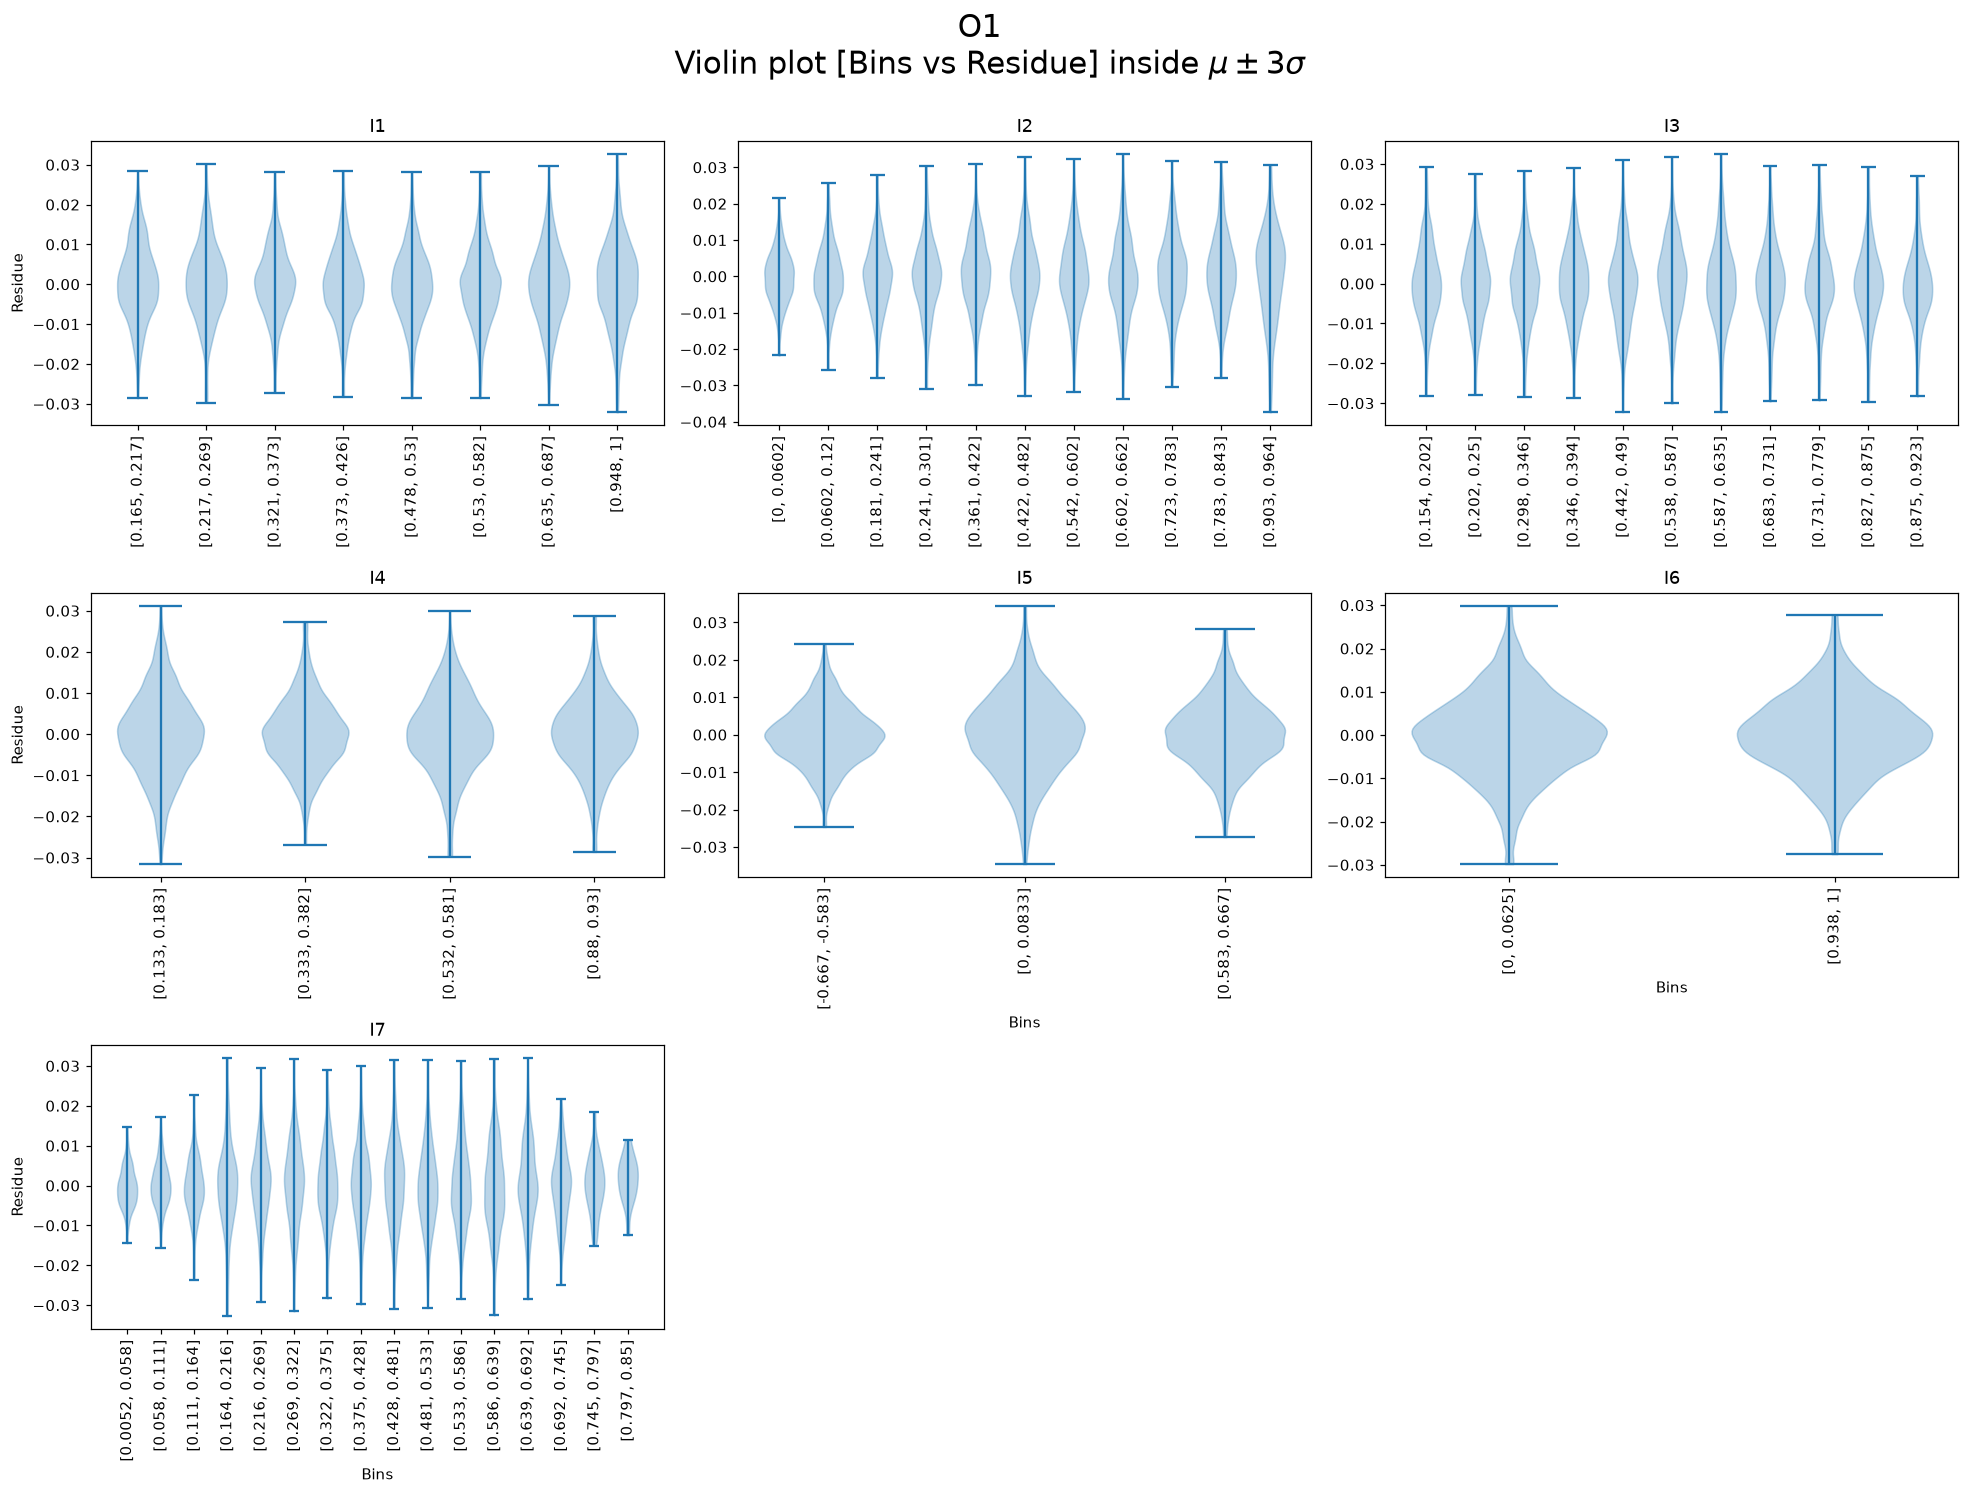
\includegraphics[width=1.0\linewidth,height=0.80\textheight,keepaspectratio]{analysis_plots/pex_violin_res_O1.png}\end{center}
\end{minipage}\par\medskip
\par\begin{minipage}{\linewidth}
\subsection*{\normalsize Residue --- O2}
\begin{center}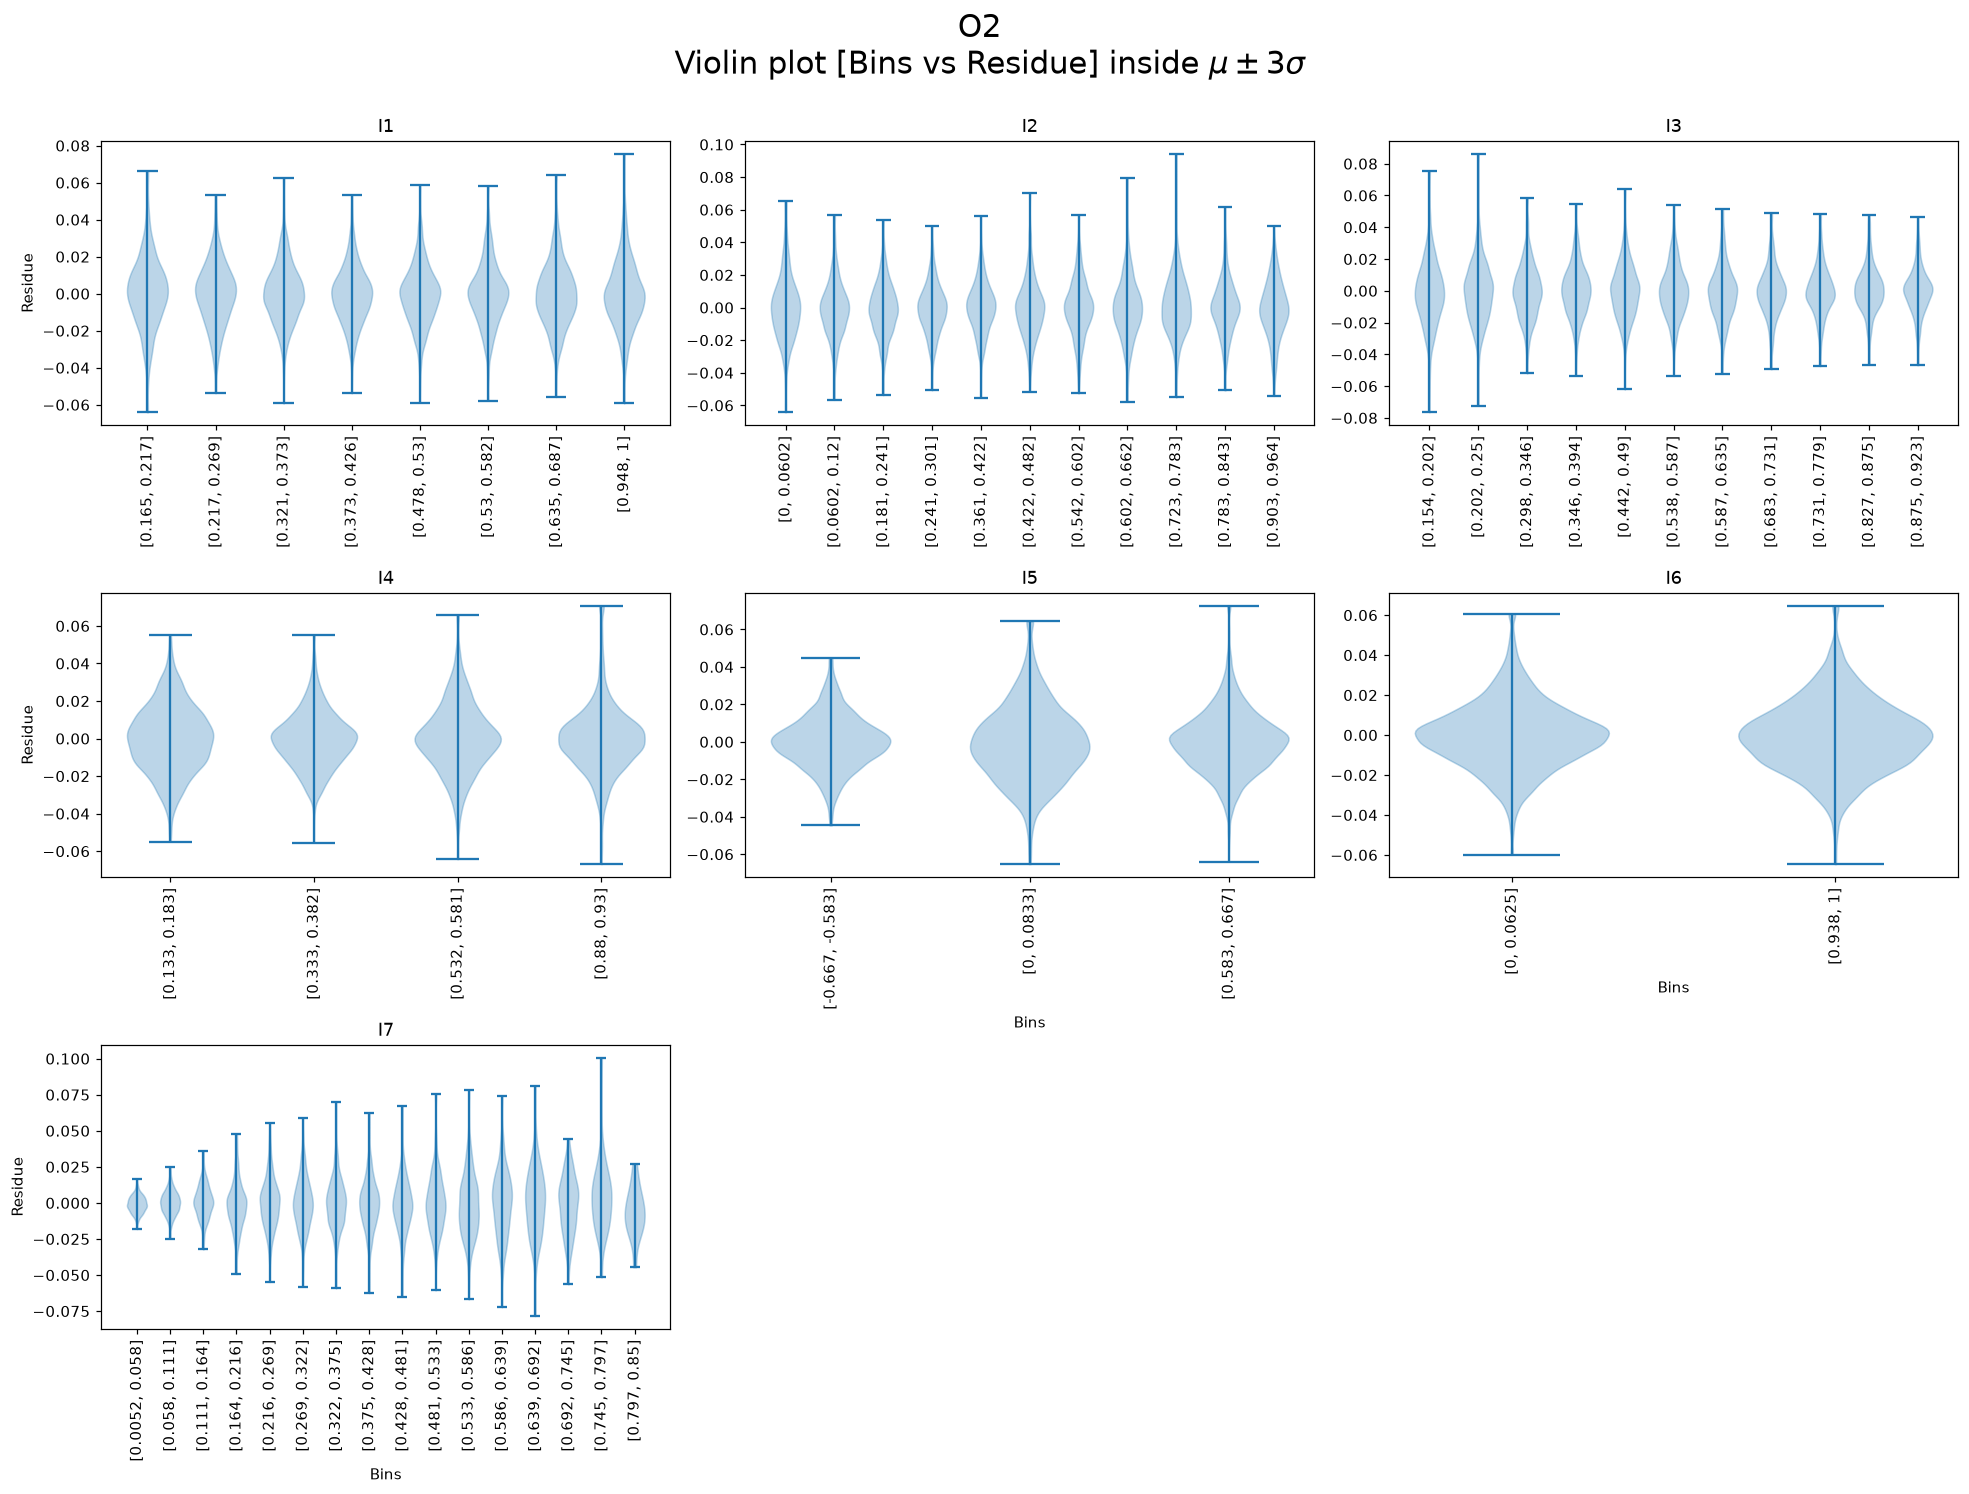
\includegraphics[width=1.0\linewidth,height=0.80\textheight,keepaspectratio]{analysis_plots/pex_violin_res_O2.png}\end{center}
\end{minipage}\par\medskip
\clearpage
\exhead{Absolute Error Violin Plots per Output (binned by input)}
\par\begin{minipage}{\linewidth}
\subsection*{\normalsize Absolute Error --- O1}
\begin{center}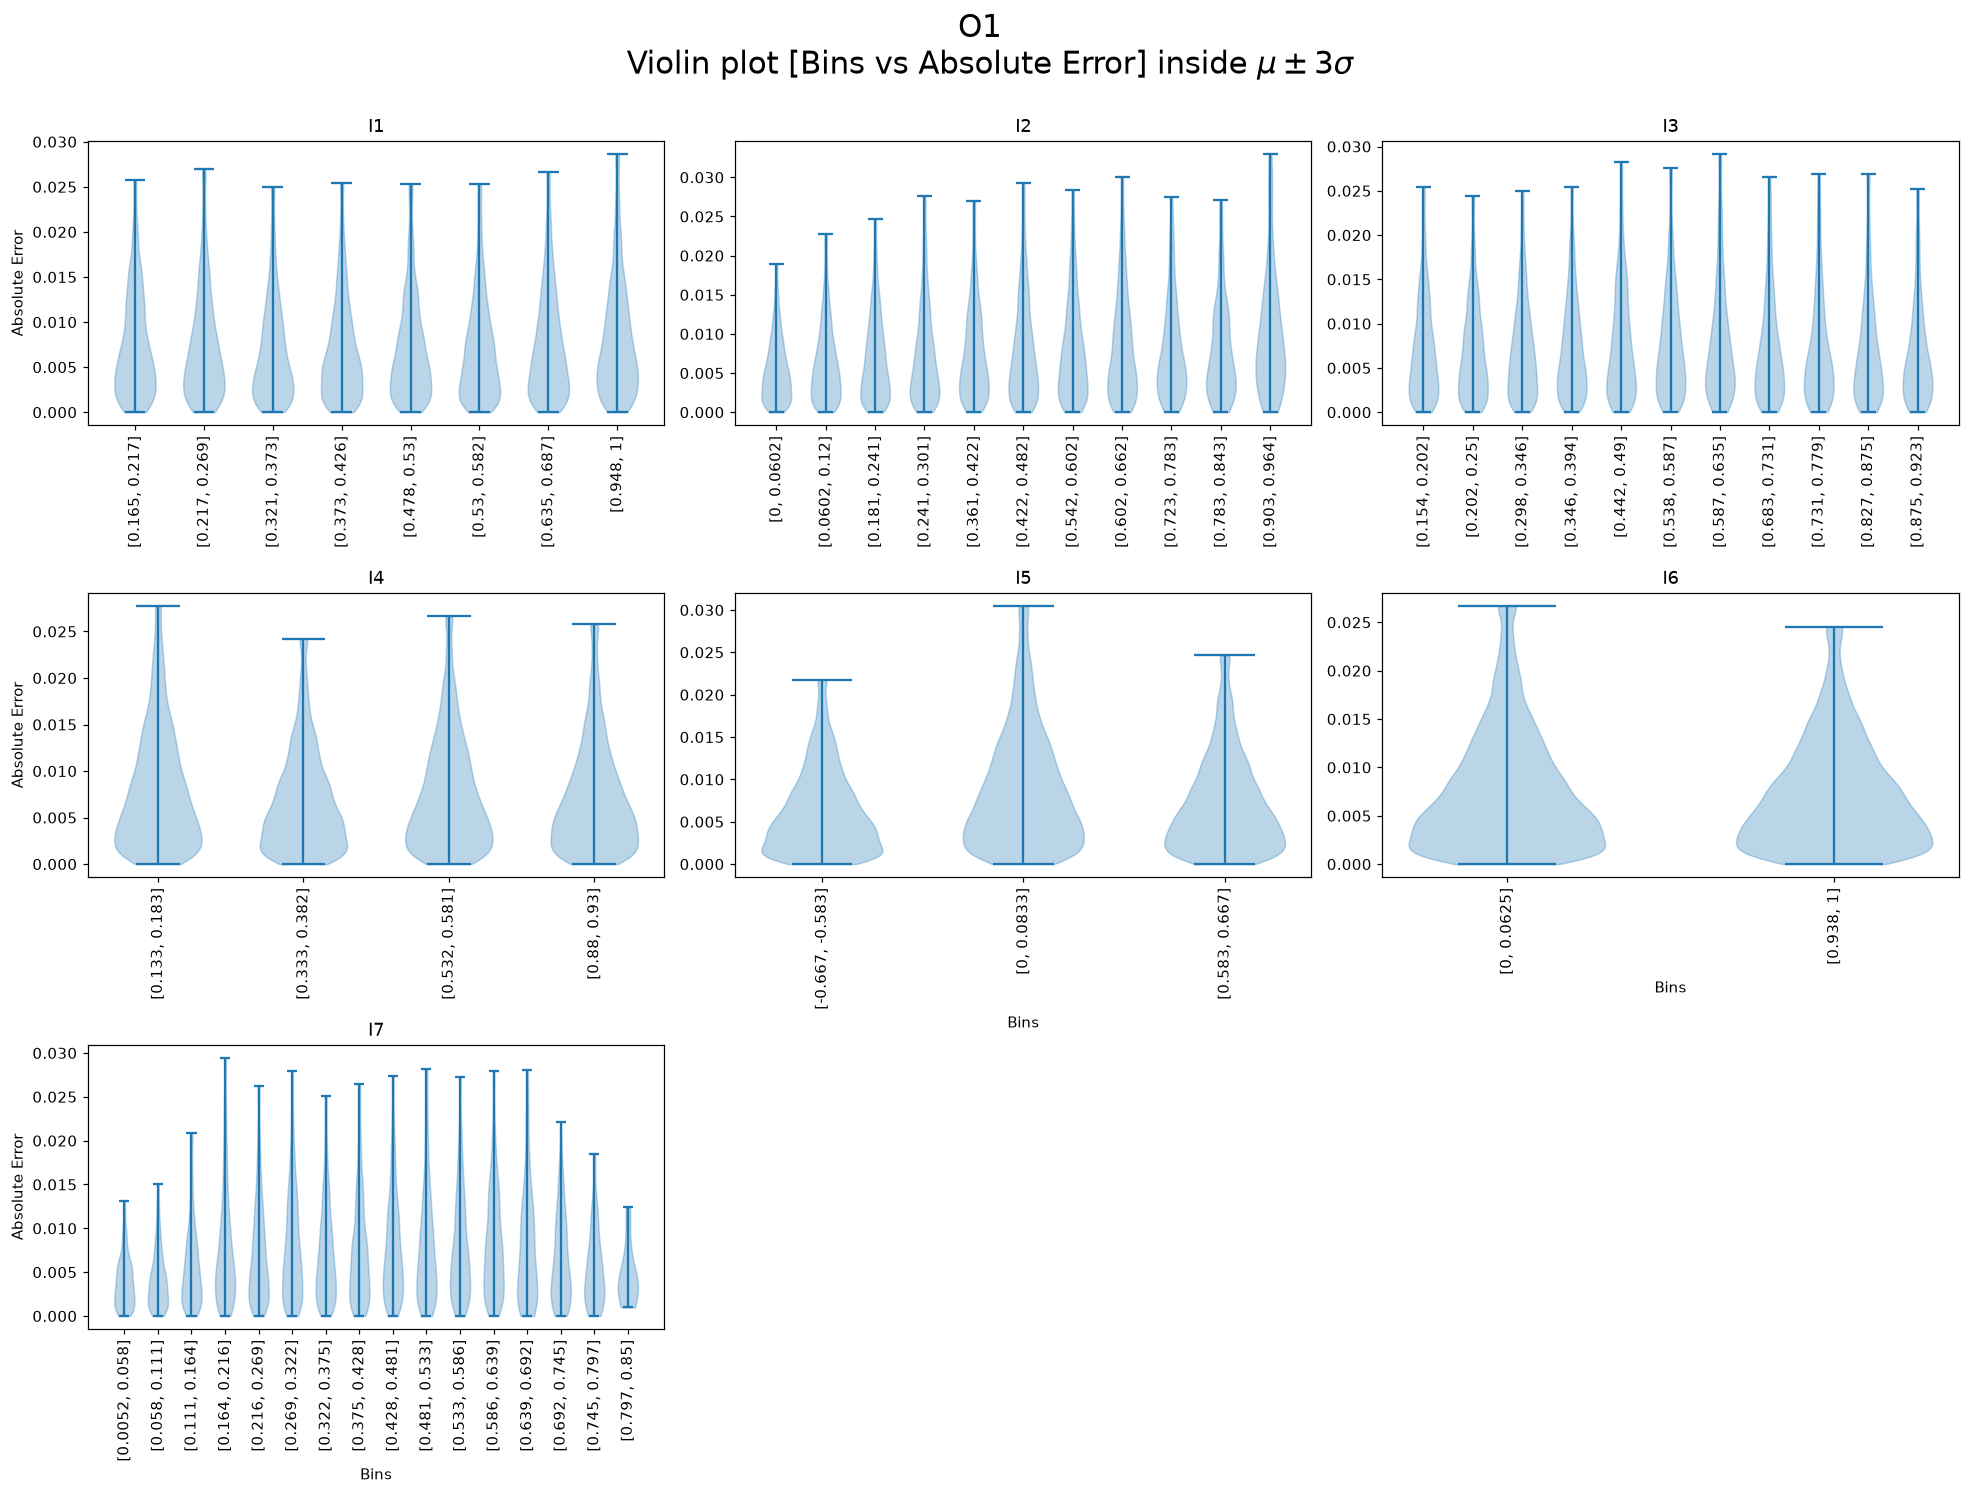
\includegraphics[width=1.0\linewidth,height=0.80\textheight,keepaspectratio]{analysis_plots/pex_violin_abs_O1.png}\end{center}
\end{minipage}\par\medskip
\par\begin{minipage}{\linewidth}
\subsection*{\normalsize Absolute Error --- O2}
\begin{center}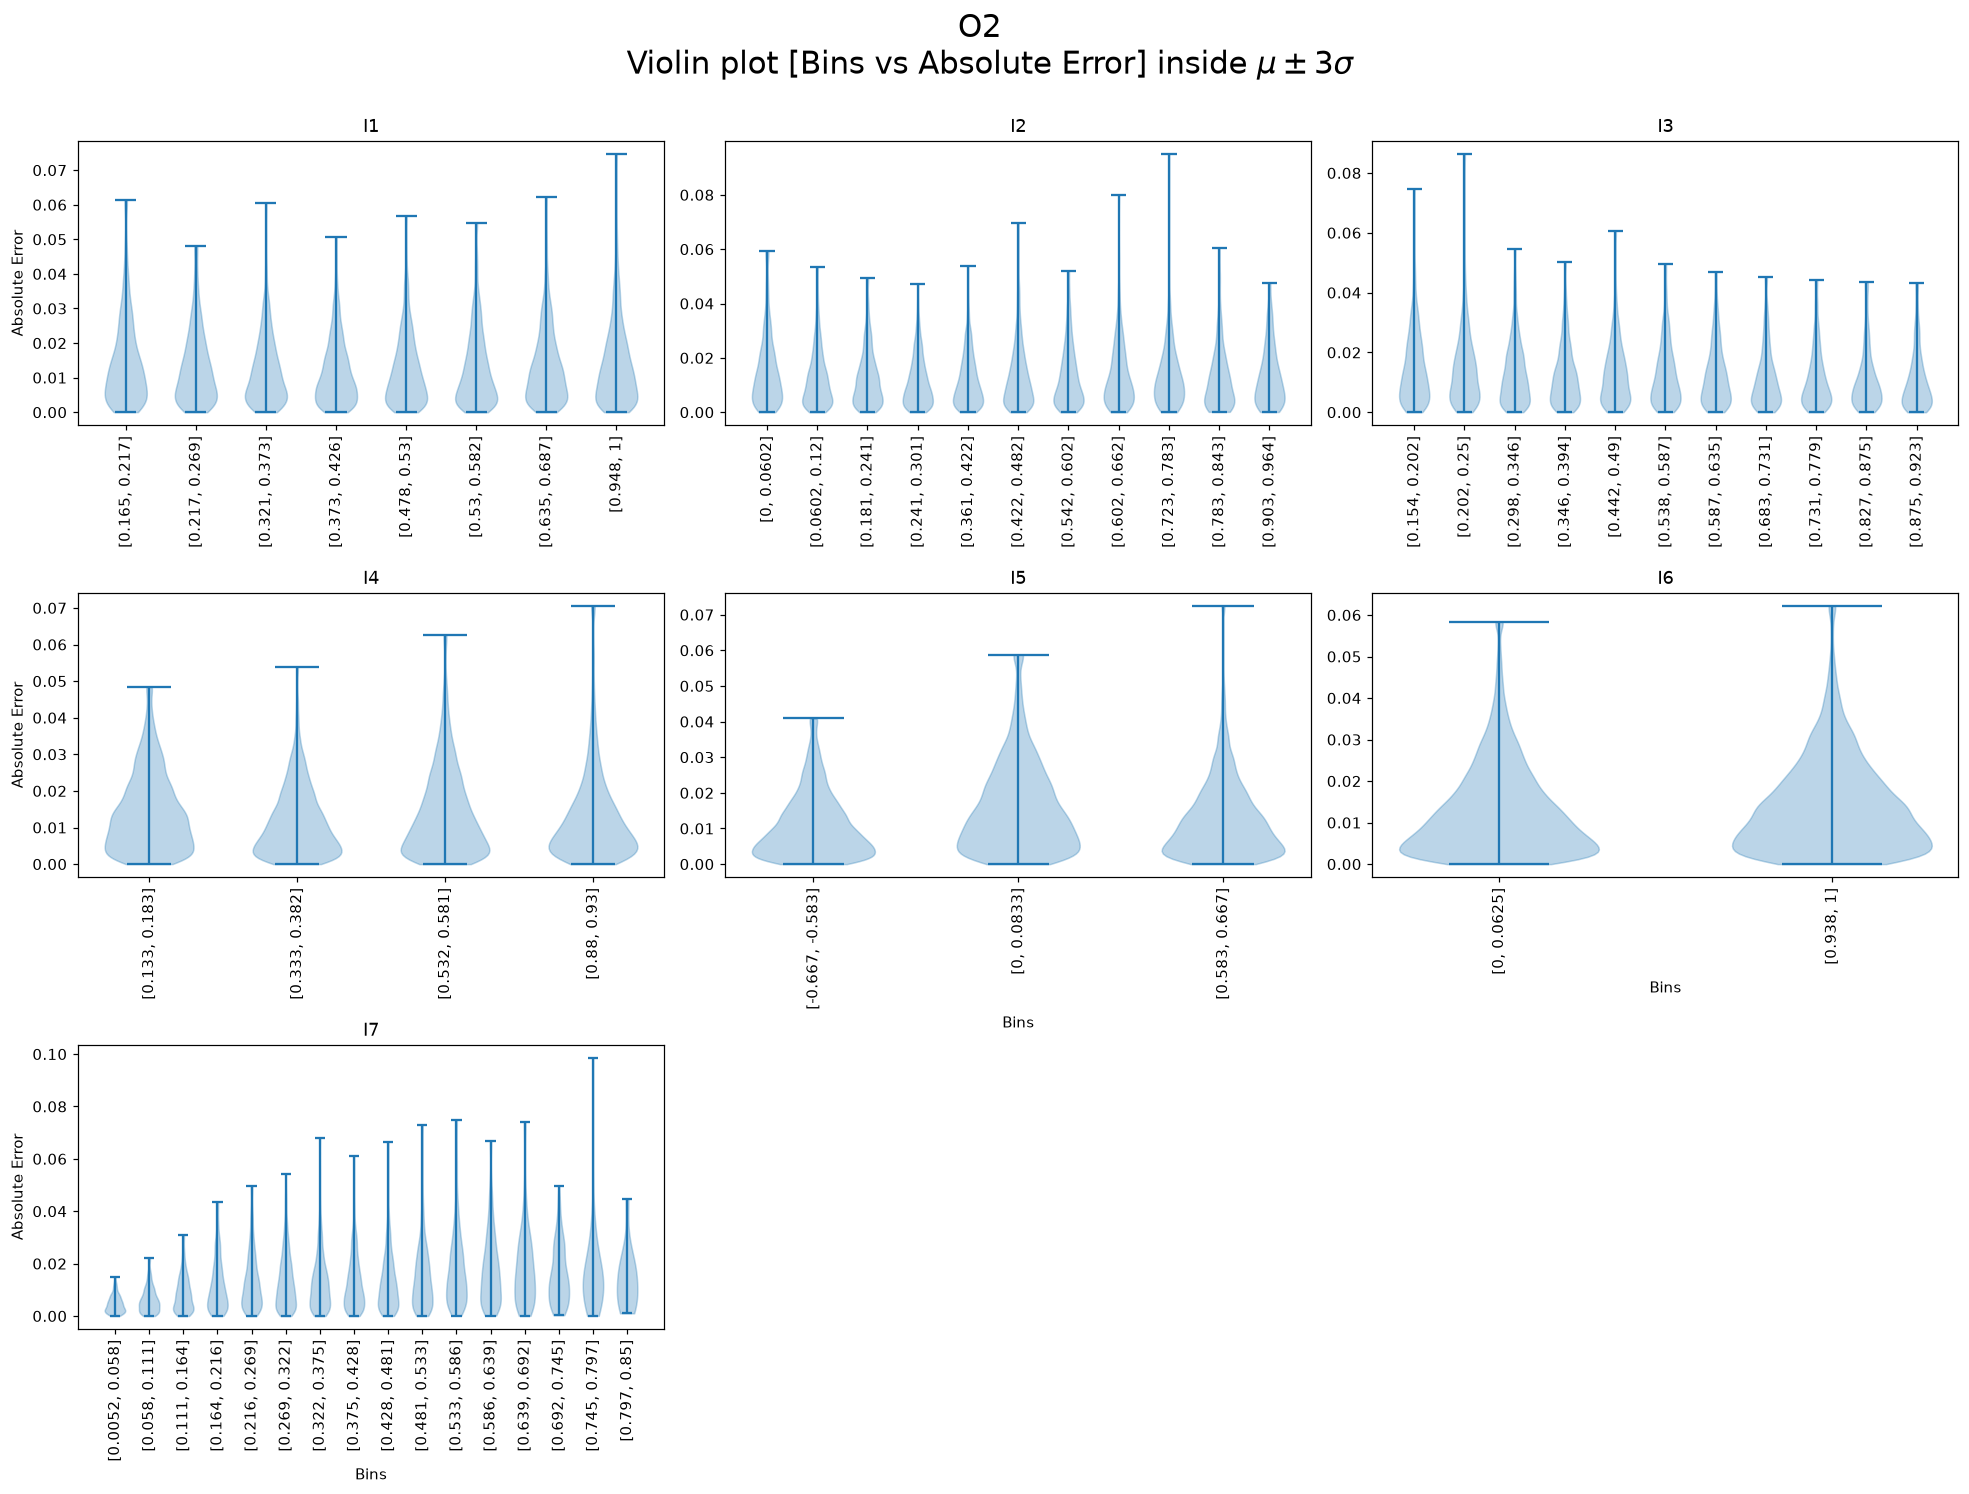
\includegraphics[width=1.0\linewidth,height=0.80\textheight,keepaspectratio]{analysis_plots/pex_violin_abs_O2.png}\end{center}
\end{minipage}\par\medskip
\clearpage
\section{P(E|Y) --- Error Conditional on Outputs}
\label{sec:d5}

We study whether the error depends on the output magnitude. A significant trend (Pearson or Spearman $p<0.05$) means the model is more accurate in some output ranges than others --- a form of heteroscedasticity.

\par\begin{minipage}{\linewidth}
\exhead{Residue vs True Output --- Scatter}
The legend shows the least-squares fit and its R\textsuperscript{2}.
\begin{center}
\includegraphics[width=1.0\linewidth,height=0.80\textheight,keepaspectratio]{analysis_plots/pey_residue_scatter.png}\end{center}
\end{minipage}\par\medskip
\par\begin{minipage}{\linewidth}
\exhead{Residue Trend Tests (Pearson / Spearman)}
Each output's residue against its own true value, as the extended validation notebook computes them: correlation coefficient, trend-test p-value ($p<0.05$ = significant trend) and, for Pearson, the normalized slope. The full cross-output tables are in the extended validation HTML.
\begin{center}
\footnotesize
\renewcommand{\arraystretch}{1.15}
\begin{tabular}{|l|r|r|}
\hline
\textbf{} & \textbf{O1} & \textbf{O2} \\ \hline
\textbf{Pearson coeff.} & 0.0827 & 0.2126 \\ \hline
\textbf{p-value} & 1.79e-28 & 7.81e-182 \\ \hline
\textbf{Slope (normalized)} & 0.05 & 0.0561 \\ \hline
\end{tabular}
\par\vspace{2pt}
{\scriptsize Residue vs.\ its true output --- Pearson trend test}
\end{center}
\begin{center}
\footnotesize
\renewcommand{\arraystretch}{1.15}
\begin{tabular}{|l|r|r|}
\hline
\textbf{} & \textbf{O1} & \textbf{O2} \\ \hline
\textbf{Spearman coeff.} & 0.0759 & 0.1545 \\ \hline
\textbf{p-value} & 3.07e-24 & 6.05e-96 \\ \hline
\end{tabular}
\par\vspace{2pt}
{\scriptsize Residue vs.\ its true output --- Spearman trend test}
\end{center}
\end{minipage}\par\medskip
\par\begin{minipage}{\linewidth}
\exhead{Residue Violin vs True Output Bins}
Bins determined by Sturges rule. Median line dashed at 0.
\begin{center}
\includegraphics[width=1.0\linewidth,height=0.80\textheight,keepaspectratio]{analysis_plots/pey_residue_violin.png}\end{center}
\end{minipage}\par\medskip
\par\begin{minipage}{\linewidth}
\exhead{Absolute Error vs True Output --- Scatter}
The legend shows the least-squares fit and its R\textsuperscript{2}.
\begin{center}
\includegraphics[width=1.0\linewidth,height=0.80\textheight,keepaspectratio]{analysis_plots/pey_abserr_scatter.png}\end{center}
\end{minipage}\par\medskip
\par\begin{minipage}{\linewidth}
\exhead{Absolute Error Trend Tests (Pearson / Spearman)}
\begin{center}
\footnotesize
\renewcommand{\arraystretch}{1.15}
\begin{tabular}{|l|r|r|}
\hline
\textbf{} & \textbf{O1} & \textbf{O2} \\ \hline
\textbf{Pearson coeff.} & 0.1398 & 0.2703 \\ \hline
\textbf{p-value} & 1.04e-78 & 7.57e-297 \\ \hline
\textbf{Slope (normalized)} & 0.106 & 0.063 \\ \hline
\end{tabular}
\par\vspace{2pt}
{\scriptsize Absolute error vs.\ its true output --- Pearson trend test}
\end{center}
\begin{center}
\footnotesize
\renewcommand{\arraystretch}{1.15}
\begin{tabular}{|l|r|r|}
\hline
\textbf{} & \textbf{O1} & \textbf{O2} \\ \hline
\textbf{Spearman coeff.} & 0.1383 & 0.2364 \\ \hline
\textbf{p-value} & 4.37e-77 & 1.6e-225 \\ \hline
\end{tabular}
\par\vspace{2pt}
{\scriptsize Absolute error vs.\ its true output --- Spearman trend test}
\end{center}
\end{minipage}\par\medskip
\par\begin{minipage}{\linewidth}
\exhead{Absolute Error Violin vs True Output Bins}
\begin{center}
\includegraphics[width=1.0\linewidth,height=0.80\textheight,keepaspectratio]{analysis_plots/pey_abserr_violin.png}\end{center}
\end{minipage}\par\medskip
\clearpage
\section{Uncertainty Analysis}
\label{sec:d6}

A global binned uncertainty model (95th percentile, right-tailed) is trained on the validation split of the absolute error and evaluated on the held-out test split, as in the extended validation notebook. Coverage is the proportion of test points whose error falls inside the predicted bound; it should be close to 95\%.

\par\begin{minipage}{\linewidth}
\exhead{Coverage Plot}
\begin{center}
\includegraphics[width=1.0\linewidth,height=0.80\textheight,keepaspectratio]{analysis_plots/uncertainty_coverage.png}\end{center}
\end{minipage}\par\medskip
\exhead{Coverage Table}
\begin{center}
\footnotesize
\renewcommand{\arraystretch}{1.15}
\begin{tabular}{|l|r|r|r|}
\hline
\textbf{} & \textbf{O1} & \textbf{O2} & \textbf{TOTAL COV} \\ \hline
\textbf{Coverage} & 94.79 & 95.12 & \textemdash \\ \hline
\textbf{CI} & [94.45, 95.11] & [94.79, 95.43] & \textemdash \\ \hline
\end{tabular}
\par\vspace{2pt}
{\scriptsize Empirical coverage of the 95th-percentile uncertainty bound on the test split.}
\end{center}

\end{document}
